
\documentclass[11pt,oneside, a4paper]{amsart}\usepackage[]{graphicx}\usepackage[]{color}
%% maxwidth is the original width if it is less than linewidth
%% otherwise use linewidth (to make sure the graphics do not exceed the margin)
\makeatletter
\def\maxwidth{ %
  \ifdim\Gin@nat@width>\linewidth
    \linewidth
  \else
    \Gin@nat@width
  \fi
}
\makeatother

\definecolor{fgcolor}{rgb}{0.345, 0.345, 0.345}
\newcommand{\hlnum}[1]{\textcolor[rgb]{0.686,0.059,0.569}{#1}}%
\newcommand{\hlstr}[1]{\textcolor[rgb]{0.192,0.494,0.8}{#1}}%
\newcommand{\hlcom}[1]{\textcolor[rgb]{0.678,0.584,0.686}{\textit{#1}}}%
\newcommand{\hlopt}[1]{\textcolor[rgb]{0,0,0}{#1}}%
\newcommand{\hlstd}[1]{\textcolor[rgb]{0.345,0.345,0.345}{#1}}%
\newcommand{\hlkwa}[1]{\textcolor[rgb]{0.161,0.373,0.58}{\textbf{#1}}}%
\newcommand{\hlkwb}[1]{\textcolor[rgb]{0.69,0.353,0.396}{#1}}%
\newcommand{\hlkwc}[1]{\textcolor[rgb]{0.333,0.667,0.333}{#1}}%
\newcommand{\hlkwd}[1]{\textcolor[rgb]{0.737,0.353,0.396}{\textbf{#1}}}%

\usepackage{framed}
\makeatletter
\newenvironment{kframe}{%
 \def\at@end@of@kframe{}%
 \ifinner\ifhmode%
  \def\at@end@of@kframe{\end{minipage}}%
  \begin{minipage}{\columnwidth}%
 \fi\fi%
 \def\FrameCommand##1{\hskip\@totalleftmargin \hskip-\fboxsep
 \colorbox{shadecolor}{##1}\hskip-\fboxsep
     % There is no \\@totalrightmargin, so:
     \hskip-\linewidth \hskip-\@totalleftmargin \hskip\columnwidth}%
 \MakeFramed {\advance\hsize-\width
   \@totalleftmargin\z@ \linewidth\hsize
   \@setminipage}}%
 {\par\unskip\endMakeFramed%
 \at@end@of@kframe}
\makeatother

\definecolor{shadecolor}{rgb}{.97, .97, .97}
\definecolor{messagecolor}{rgb}{0, 0, 0}
\definecolor{warningcolor}{rgb}{1, 0, 1}
\definecolor{errorcolor}{rgb}{1, 0, 0}
\newenvironment{knitrout}{}{} % an empty environment to be redefined in TeX

\usepackage{alltt}
\usepackage{natbib}

\usepackage{amsbsy,amsmath}
\usepackage{amssymb,amsfonts}
\usepackage{bbm}%give 1 with dbl vertical bar 
\usepackage{booktabs,url,enumerate}
\usepackage{color,xcolor,colortbl}
\usepackage{float}
\usepackage{tikz}
\usepackage{rotating,graphicx,lscape}
\usepackage{commath}
\usetikzlibrary{arrows,positioning} 
\usepackage[hypcap]{caption}
\newcommand{\sgn}{\mathrm{sign}}
\usepackage{setspace}

% bold rows
\usepackage{array}
\newcolumntype{$}{>{\global\let\currentrowstyle\relax}}
\newcolumntype{^}{>{\currentrowstyle}}
\newcommand{\rowstyle}[1]{\gdef\currentrowstyle{#1}%
  #1\ignorespaces
}

% Invisible table columns!
\newcolumntype{H}{>{\setbox0=\hbox\bgroup}c<{\egroup}@{}}% Properly placed sideways table with asmart class. 

\setlength\rotFPtop{0pt plus 1fil} 


\usepackage[top=1.5cm, bottom=1.5cm, left=3.0cm, right=3.0cm]{geometry}

\DeclareMathOperator{\Med}{\mathbb{M}ed}
\DeclareMathOperator{\Mean}{\mathbb{M}ean}
\DeclareMathOperator{\Cov}{\mathbb{C}ov}
\DeclareMathOperator{\Var}{\mathbb{V}ar}
\DeclareMathOperator{\E}{\mathbb{E}}
\DeclareMathOperator{\nid}{NID}
\DeclareMathOperator{\N}{\mathcal{N}}
\DeclareMathOperator{\corr}{corr}
\DeclareMathOperator{\diag}{diag}
\onehalfspace


\definecolor{LightRed}{rgb}{1,.88,.88}
\definecolor{LightBlue}{rgb}{.88,.88,1}
\definecolor{LightGreen}{rgb}{.88,1,.88}

\newtheorem{theorem}{Theorem}
\IfFileExists{upquote.sty}{\usepackage{upquote}}{}
\begin{document}
	
\title{Some notes on VAR models for the EZ.}   
\author{LAFC}
\date{\today}
\maketitle

Define a set of endogenous variables $Y_t=[y_{1t},...,y_{k_Y t}]$, $t=1,...,T$, and define a set of exogenous variables $X_t$ stored in vectors of dimension $1\times k_Y$ and $1\times k_X$, respectively. Note that $Y_t$ could be the first difference of some variables, I use this notation for the sake of generality. Let $D_t$ be the vector of deterministic components of the model. $D_t$ could contain an intercept, a linear trend, or dummies. Also define $Z_t'=[Y_{t-1}',...,Y_{t-p}',X_{t}',D_t']$. The main model we consider is a VARX(p) of the form
\begin{align}
 Y_t &= D_t^* + \sum_{l=1}^p  Y_{t-l}A_l^* + X_t B^* + \epsilon_t,\nonumber\\
    &= D_t^* + Z_t \Gamma^* + \epsilon_t^*,\nonumber\\
 y_{it}&= d_{it}^* + Z_{t} \gamma_i^* + \epsilon_{it}^*,\label{eq:var}
\end{align}
The parameter matrix $\Gamma^*$ is of dimensions $ k_Y \times \left(pk_Y+k_X (:=k) \right)$. The VAR is estimated equation-by-equation both to speed up computations and to adapt the penalty to the variance in each equation. A possible exception is if using the group Lasso for lag selection.   


\section*{Estimation}

\subsection*{Lasso}
The objective function of the Lasso is given by 
\begin{align}
L(\gamma_{i})=\frac{1}{T}\enVert{y_{i}-d_{it}-Z\gamma_{i}}^2+2\lambda_T\enVert{\gamma_{i}}_{\ell_1}\label{eq:obj}.
\end{align}

The model is estimated equation-by-equation and the penalty parameter is selected by BIC among those on the path selected by \texttt{glmnet}. \texttt{Lassovar} takes care of this part.  

\subsection*{Adaptive Lasso}

The objective function of the adaptive Lasso is given by 
\begin{align}
L(\gamma_{i})=\frac{1}{T}\enVert{y_{i}-d_{it}-Z\gamma_{i}}^2+2\lambda_T\sum_{j=1}^{k}w_{ij}\gamma_{ij}\label{eq:objada}.
\end{align}
where the adaptive weights can be given by $w_{ij}=\frac{1}{\hat\gamma_{ij}}$ where $\hat\gamma_{ij}$ is some initial estimator of $\gamma^*_{ij}$. If $\hat\gamma_{ij}=0$, variable $j$ is excluded from equation $i$ before estimating the adaptive Lasso. OLS or the Lasso are fine initial estimators, but they both have weaknesses. The risk of misclassification for the Lasso (excluding a relevant variable) and the poor quality of the estimates if $k$ is close to $T$.    



\section*{Shock response}

Consider a VAR(1) in difference where the parameters have been estimated:
\begin{align}
\Delta Y_t &= \Delta Y_{t-1} \hat A + \epsilon_t,\nonumber
\end{align}

To compute the response to an exogenous shock of size $s$ to the first variable in $Y$, construct the vector $\delta =[s,0,...,0]$. The response at after $h$ periods is given by $\delta \hat A^h$. 
\begin{itemize}
\item For models with multiple lags the companion form (or simply recursive computations) can be used.
\item For models with exogenous variables, at path for the exogenous variables has to be specified. In general it should be equal to zero or to a random walk forecast, at least in periods following an initial shock. 
\item The deterministics can be omitted. 
\item For VECM models, things are more complicated but not much more difficult.    
\end{itemize}


\section*{Conditional forecasts}

The options so far:
\begin{itemize}
\item Create a model for the exogenous variable. 
\item Use na\"{i}ve methods (i.e. RW).
\item Compute prediction density for the exogenous variable and plug in the model. Gaussian + linear = Gaussian.
\item Condition on true value. 
\end{itemize}



\section*{Some tests}


\begin{knitrout}
\definecolor{shadecolor}{rgb}{0.969, 0.969, 0.969}\color{fgcolor}\begin{kframe}
\begin{alltt}
\hlkwd{library}\hlstd{(}\hlstr{'lassovar'}\hlstd{)}
\hlkwd{library}\hlstd{(}\hlstr{'ggplot2'}\hlstd{)}
\hlkwd{load}\hlstd{(}\hlstr{'../Result/vardata'}\hlstd{)}
\hlcom{# loadind and subseting the data}
\hlstd{dat} \hlkwb{<-} \hlkwd{data.frame}\hlstd{(vardataframe[}\hlnum{116}\hlopt{:}\hlnum{180}\hlstd{,} \hlkwd{c}\hlstd{(}\hlnum{1}\hlstd{,}\hlnum{2}\hlstd{,}\hlnum{6}\hlstd{,}\hlnum{11}\hlstd{,}\hlnum{13}\hlstd{,}\hlnum{17}\hlstd{,}\hlnum{8}\hlstd{,}\hlnum{24}\hlstd{) ])}
\hlcom{# differentiating}
\hlstd{difdat} \hlkwb{<-} \hlkwd{tail}\hlstd{(dat,}\hlopt{-}\hlnum{1}\hlstd{)} \hlopt{-} \hlkwd{head}\hlstd{(dat,}\hlopt{-}\hlnum{1}\hlstd{)}
\end{alltt}
\end{kframe}
\end{knitrout}

\begin{knitrout}
\definecolor{shadecolor}{rgb}{0.969, 0.969, 0.969}\color{fgcolor}\begin{kframe}
\begin{alltt}
\hlcom{# estimate a VAR(1)}
\hlstd{lv_lev}\hlkwb{<-}\hlkwd{lassovar}\hlstd{(dat,}\hlkwc{lags}\hlstd{=}\hlnum{1}\hlstd{,} \hlkwc{ic}\hlstd{=}\hlstr{"BIC"}\hlstd{)}
\hlkwd{summary}\hlstd{(lv_lev)}
\end{alltt}
\begin{verbatim}
## Call:
## lassovar(dat = dat, lags = 1, ic = "BIC")
## 
## Model estimated equation by equation
## Selection criterion: BIC
## Estimator: Lasso
## Deterministics: intercept.
## Dimensions: T = 64  N = 8
## 
## Total number of variables selected:26 (40.625% of candidates)
## 
##  Model summary statistics:
##            Lambda non-zero    resid var
## CPE   0.009137410        3 1.679413e-04
## DJES  0.047738176        3 7.856802e+01
## HICP  0.002310290        4 2.891006e-04
## LTN   0.006771786        3 6.916725e-02
## M3    0.014432675        3 1.286696e-03
## POILU 0.037676144        4 2.943369e-01
## LHO   0.018900280        1 1.011330e-03
## YED   0.007223302        5 1.002183e-04
## 
## Deterministics not included in the non-zero count.
\end{verbatim}
\begin{alltt}
\hlstd{lv_lev_trend}\hlkwb{<-}\hlkwd{lassovar}\hlstd{(dat,}\hlkwc{lags}\hlstd{=}\hlnum{1}\hlstd{,} \hlkwc{ic}\hlstd{=}\hlstr{"BIC"}\hlstd{,}\hlkwc{exo}\hlstd{=}\hlkwd{seq}\hlstd{(}\hlnum{1}\hlopt{:}\hlkwd{nrow}\hlstd{(dat)))}
\hlkwd{summary}\hlstd{(lv_lev_trend)}
\end{alltt}
\begin{verbatim}
## Call:
## lassovar(dat = dat, exo = seq(1:nrow(dat)), lags = 1, ic = "BIC")
## 
## Model estimated equation by equation
## Selection criterion: BIC
## Estimator: Lasso
## Deterministics: intercept.
## Dimensions: T = 64  N = 8
## 
## Total number of variables selected:30 (41.66667% of candidates)
## 
##  Model summary statistics:
##            Lambda non-zero    resid var
## CPE   0.009137410        4 1.667344e-04
## DJES  0.052392590        4 7.243895e+01
## HICP  0.002310290        5 2.821701e-04
## LTN   0.006771786        3 6.916725e-02
## M3    0.014432675        3 1.286696e-03
## POILU 0.009332668        5 2.867100e-01
## LHO   0.018900280        1 1.011330e-03
## YED   0.007223302        5 1.002183e-04
## 
## Deterministics not included in the non-zero count.
\end{verbatim}
\begin{alltt}
\hlstd{lv_dif}\hlkwb{<-}\hlkwd{lassovar}\hlstd{(difdat,}\hlkwc{lags}\hlstd{=}\hlnum{1}\hlstd{,} \hlkwc{ic}\hlstd{=}\hlstr{"BIC"}\hlstd{)}
\hlkwd{summary}\hlstd{(lv_dif)}
\end{alltt}
\begin{verbatim}
## Call:
## lassovar(dat = difdat, lags = 1, ic = "BIC")
## 
## Model estimated equation by equation
## Selection criterion: BIC
## Estimator: Lasso
## Deterministics: intercept.
## Dimensions: T = 63  N = 8
## 
## Total number of variables selected:16 (25% of candidates)
## 
##  Model summary statistics:
##             Lambda non-zero    resid var
## CPE   0.0024551858        0 8.912461e-05
## DJES  1.8958393270        2 8.264576e+01
## HICP  0.0014289972        4 2.665823e-04
## LTN   0.0778170470        0 8.896670e-02
## M3    0.0009786965        6 8.803950e-04
## POILU 0.1861160585        0 3.695596e-01
## LHO   0.0029187219        2 2.666321e-04
## YED   0.0014462239        2 4.939361e-05
## 
## Deterministics not included in the non-zero count.
\end{verbatim}
\end{kframe}
\end{knitrout}


\begin{knitrout}
\definecolor{shadecolor}{rgb}{0.969, 0.969, 0.969}\color{fgcolor}\begin{kframe}
\begin{alltt}
\hlcom{# printing the diagonal of the parameter matrix}
\hlstd{ar1} \hlkwb{<-} \hlkwd{cbind}\hlstd{(}\hlkwd{diag}\hlstd{(}\hlkwd{coef}\hlstd{(lv_lev)[}\hlopt{-}\hlnum{1}\hlstd{,]),}
             \hlkwd{diag}\hlstd{(}\hlkwd{coef}\hlstd{(lv_lev_trend)[}\hlnum{2}\hlopt{:}\hlstd{(}\hlnum{1}\hlopt{+}\hlkwd{ncol}\hlstd{(dat)),]),}
             \hlkwd{diag}\hlstd{(}\hlkwd{coef}\hlstd{(lv_dif)[}\hlopt{-}\hlnum{1}\hlstd{,]))}


\hlkwd{rownames}\hlstd{(ar1)} \hlkwb{<-} \hlstd{lv_lev}\hlopt{$}\hlstd{var.names}
\hlkwd{colnames}\hlstd{(ar1)} \hlkwb{<-} \hlkwd{c}\hlstd{(}\hlstr{'level'}\hlstd{,}\hlstr{'level + trend'}\hlstd{,}\hlstr{'diff'}\hlstd{)}
\hlstd{mar1} \hlkwb{<-} \hlkwd{melt}\hlstd{(ar1)}

\hlkwd{ggplot}\hlstd{(mar1,}\hlkwd{aes}\hlstd{(}\hlkwc{x}\hlstd{=Var1,}\hlkwc{y}\hlstd{=value,}\hlkwc{colour}\hlstd{=Var2,}\hlkwc{shape}\hlstd{=Var2))} \hlopt{+}
  \hlkwd{geom_point}\hlstd{(}\hlkwc{size}\hlstd{=}\hlnum{3}\hlstd{)} \hlopt{+} \hlkwd{theme_minimal}\hlstd{()}
\end{alltt}
\end{kframe}
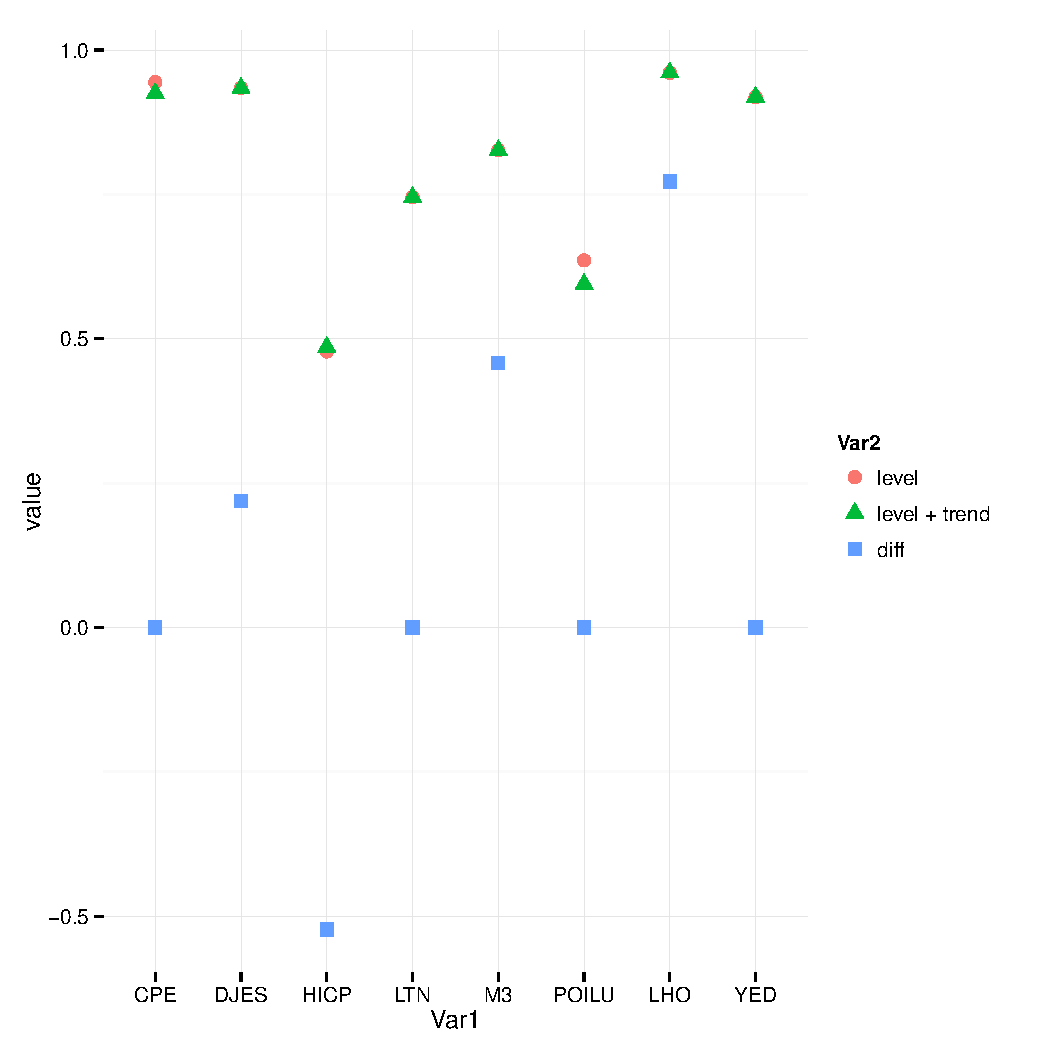
\includegraphics[width=\maxwidth]{figure/plotar-1} 

\end{knitrout}


The parameters fo the VAR in level are pretty close to 1. The trend is usually set to zero by the Lasso. It should probably not be penalized anyway. In the model in difference, the estimator often does not select an equation's own lag in most cases. weird. 


\end{document}
